\documentclass[12pt,a4paper]{article}

\usepackage[utf8]{inputenc}
\usepackage[english]{babel}
\usepackage{amsmath}
\usepackage{amsfonts}
\usepackage{amssymb}
\usepackage{graphicx}
\usepackage{lmodern}
\usepackage[left=2cm,right=2cm,top=2cm,bottom=2cm]{geometry}

\usepackage{siunitx}
\usepackage{enumitem}
\usepackage[skip=.38\baselineskip]{parskip}
\usepackage{xcolor}   % for \textcolor
\usepackage{listings}
\definecolor{mGreen}{rgb}{0,0.4,0.1}
\definecolor{mGray}{rgb}{0.5,0.5,0.5}
\definecolor{mPurple}{rgb}{0.58,0,0.82}
\definecolor{backgroundColour}{rgb}{0.95,0.95,0.92}
\lstset{
	%backgroundcolor=\color{backgroundColour},   
    commentstyle=\color{mGreen},
    keywordstyle=\color{magenta},
    numberstyle=\tiny\color{mGray},
    stringstyle=\color{mPurple},
    %breakatwhitespace=false,                        
    %captionpos=b,
    %keepspaces=true,                 
    numbers=left,                    
    numbersep=5pt,                  
    showspaces=false,                
    showstringspaces=false,
    showtabs=false,                  
    %tabsize=8,	
    language=C,    
  	basicstyle=\small\ttfamily,
  	columns=fullflexible,
  	frame=single,
  	breaklines=true,
  	postbreak=\mbox{\textcolor{red}{$\hookrightarrow$}\space},
}

% for multi-figures
\usepackage{subcaption}

% for graphs
%\usepackage{tikz}
%\usepackage{tkz-graph}
%\input{tkz-graph-patch}
%\usepackage{tikz-qtree}
%\usetikzlibrary{calc, arrows, positioning}

% custom commands
\newcommand{\multilinecell}[1]{\begin{tabular}{@{}c@{}}#1\end{tabular}}

\author{Olivér Facklam}
\title{CS473: MSP432 laboratory\\Controlling servomotor with analog joystick}

\newcommand{\nil}{\textit{nil}}

\begin{document}
\maketitle
\tableofcontents

\section{Problem statement}

The goal of this lab is to create a system in which a servomotor's position is controlled by a joystick. We want to link the servomotor and the joystick together through some logic implemented on an MSP432 microcontroller. The servomotor's angle should follow the joystick's position.

More precisely the requirements are the following. The analog value provided by the joystick should be sampled and converted every \SI{50}{\milli\s}. The servomotor should be controlled by a pulse-width modulated signal (PWM), with a period of \SI{20}{\milli\s} and a width between \SI{1}{\milli\s} and \SI{2}{\milli\s}. The joystick value should be mapped to a PWM duty-cycle and used to update the servomotor's angle.

I decided to target a precision of 1\%.

\section{High-level system description}

The following building blocks are required to achieve the desired operation. An overview of this setup is given in a block-diagram form in figure \ref{fig:schema}.
\begin{itemize}
\item The clock system is set up to provide a sufficiently precise and high-frequency signal to drive the processor and all the subsystems. The DCO (digitally controlled oscillator) is routed to the MCLK (master clock) and SMCLK (low-speed subsystem master clock) signals.
\item Two timers are used: TIMER\_A0 is dedicated to generating the PWM signal for the servomotor control, while TIMER\_A3 is used to periodically initiate the sampling and conversion of the analog value.
\item TIMER\_A0 uses the SMCLK signal and operates in UP mode, with a period corresponding to the required PWM period, which is \SI{20}{\milli\s}. The capture-compare block CCR1 is used to set the PWM duty cycle. It operates in a RESET/SET output mode, generating the required PWM signal which is routed to pin 2.4.
\item TIMER\_A3 is set to UP mode and is used to trigger a processor interrupt at the predefined rate (every \SI{50}{\milli\s}).
\item The analog-to-digital converter (ADC) uses the SMCLK signal and pulse sample mode for the conversions. These are triggered by the processor every \SI{50}{\milli\s}. The analog channel A13 (corresponding to port 4.0) is sampled, and the value is stored in memory slot 0. A processor interrupt is triggered at the end of the conversion, allowing it to read the sampled value.
\item The processor operates with two interrupts. The interrupt from TIMER\_A3 is used to trigger the conversion process in the ADC. The interrupt from the ADC is used to read the sampled value, do some calculations and finally update the duty-cycle of the PWM in TIMER\_A0's CCR1.
\end{itemize}

\begin{figure}[h]
	\centering
	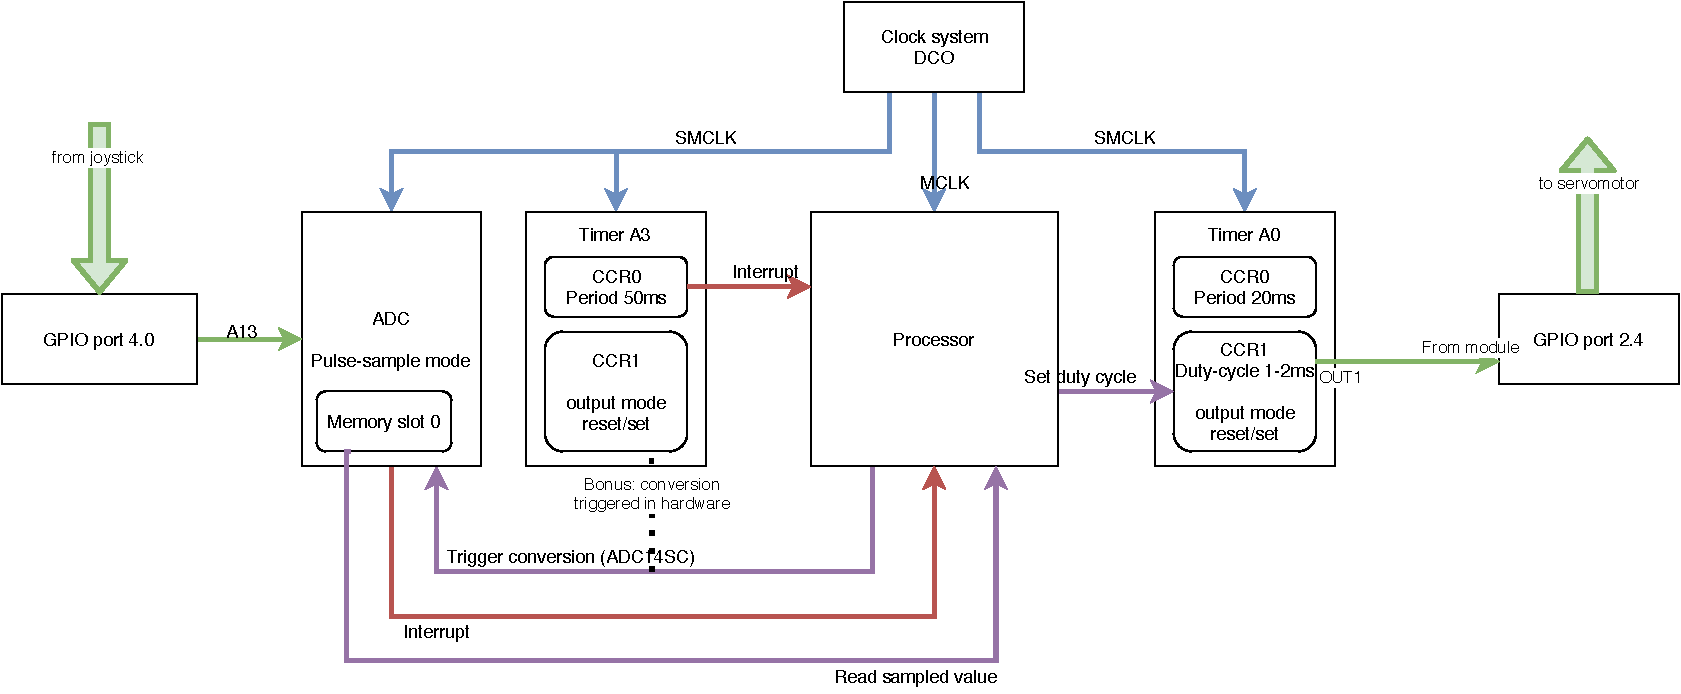
\includegraphics[width=\linewidth]{block}
	\caption{Block diagram of system operation}
	\label{fig:schema}
\end{figure}

\section{Detailed operation description}

\subsection{General setup}
The general setup is controlled by \texttt{main.c}. The function \texttt{manip\_7} implements the targeted system, with a software-triggered ADC conversion. The function \texttt{manip\_7bis} uses a timer-triggered ADC conversion.

First, in both cases the clock system is set up by configuring and linking the DCO. Then the ADC is set to the correct mode with input A13 mapped to memory slot 0. Interrupts are enabled for the ADC and the function \texttt{update\_pwm} is set as the interrupt handler. Finally PWM is set up on pin 2.4 for the servomotor.

The two versions differ in their way of triggering conversions:
\begin{itemize}
\item \texttt{manip\_7} configures a periodic interrupt which triggers the ADC conversion by software every \SI{50}{\milli\s}.
\item \texttt{manip\_7bis} creates a PWM of period \SI{50}{\milli\s} on TIMER\_A3 which directly triggers the ADC conversion.
\end{itemize}

\lstinputlisting[language=C, firstline=119, lastline=171]{src/main.c}


\subsection{Clock system}

We need a sufficiently precise and high-frequency clock signal to target a 1\% precision on the following timing constraints:
\begin{itemize}[nosep]
\item \SI{50}{\milli\s} for the sampling period
\item \SI{20}{\milli\s} for the PWM period
\item \SI{1}{\milli\s} for the PWM active time
\end{itemize}

A 1\% precision on the \SI{1}{\milli\s} active time requires a timer granularity of \SI{10}{\micro\s}. Thus I decided to configure the clock signal in the \si{\mega\hertz} range.

The digitally-controlled oscillator (DCO) operates in the \si{\mega\hertz} range. According to the device-specific datasheet, it also has an acceptable precision of 1.2\% when in external resistor mode.

So I decided to use the DCO at a frequency of \SI{4}{\mega\hertz}. It is connected to MCLK with a divider of 1, and to SMCLK with a divider of 4. This way, the processor runs at \SI{4}{\mega\hertz} and the subsystems at \SI{1}{\mega\hertz}.

The code for configuring the DCO in a generic way can be found in \texttt{time.c}.

\lstinputlisting[language=C, firstline=27, lastline=61]{src/time.c}
\bigskip

\subsection{Timers}

\subsubsection{Timer block configuration}

Both our timers need to be configured in UP mode, to allow a periodic operation (with periods of \SI{20}{\milli\s} and \SI{50}{\milli\s}).  This setup is done in the following two functions \texttt{timer\_block\_setup\_mode\_up} and \texttt{timer\_block\_setup}.
\bigskip\bigskip

\lstinputlisting[language=C, firstline=118, lastline=152]{src/time.c}

The function \texttt{calculate\_cycles} determines the number of clock cycles which correspond to the targeted period, knowing the clock frequency. It also adjusts and returns the required divider values. This dynamic scaling allows us to use period values from \SI{1}{\milli\s} up to \SI{4}{\s}.

\subsubsection{PWM generation}

Once the timer block is set up, generating a PWM is just a question of setting the correct duty cycle and output mode in one of the capture/compare registers of the timer. \texttt{timer\_pwm\_setup} initializes such a register to output mode RESET/SET, and \texttt{timer\_pwm\_duty} allows to modify the duty cycle.

\lstinputlisting[language=C, firstline=195, lastline=232]{src/time.c}

\textit{Note:} functions \texttt{pwm\_hw\_fixed\_init} and \texttt{pwm\_hw\_fixed\_update}, which are called in \texttt{main.c}, are simply wrappers around \texttt{timer\_pwm\_setup} and \texttt{timer\_pwm\_duty} respectively. They additionally configure the correct GPIO port to accept the timer module output.

\subsubsection{Timer interrupts}

Processor interrupts are configured for TIMER\_A3 by the function \texttt{periodic\_interrupt}. It sets the timer to UP mode, and enables the interrupt triggers and their handling. A pointer to a callback function is passed as an argument: this function will be called by the IRQ handler at every interrupt.

\lstinputlisting[language=C, firstline=235, lastline=282]{src/time.c}


\subsection{Precision ADC}

\subsubsection{Conversion setup}

The ADC configuration is done using two functions. The first one, called \texttt{adc\_setup}, initializes the ADC to pulse mode sampling, and then sets conversion mode, clock input, trigger signal and resolution.

\lstinputlisting[language=C, firstline=10, lastline=36]{src/adc.c}

The second one, \texttt{adc\_memory\_setup}, configures a certain memory control, links it to an input channel and enables interrupts for it.

\lstinputlisting[language=C, firstline=55, lastline=90]{src/adc.c}

\subsubsection{ADC interrupts}

The management of ADC interrupts is similar to that of timer interrupts. A function pointer to a callback can be stored to be used as the interrupt handler. At each ADC14 interrupt, the interrupt vector is analyzed to detect the interrupt reason. If it corresponds to a finished conversion, the sampled value is read from the ADC's memory control and is handed as an argument to the callback. This logic is implemented by the following snippet of code.

\lstinputlisting[language=C, firstline=102, lastline=136]{src/adc.c}


\section{Operation \& results}
\subsection{Observed results}

Table \ref{tab:results} shows the inputs and corresponding reactions in three simple cases: the two extreme positions, and the neutral position. The corresponding PWM signals on the logic analyzer are displayed in figure \ref{fig:pwm}.

\begin{table}[h]
	\centering
	\begin{tabular}{|c|c|c|c|}
		\hline 
		Situation & minimum & neutral & maximum\\ 
		\hline 
		Input & 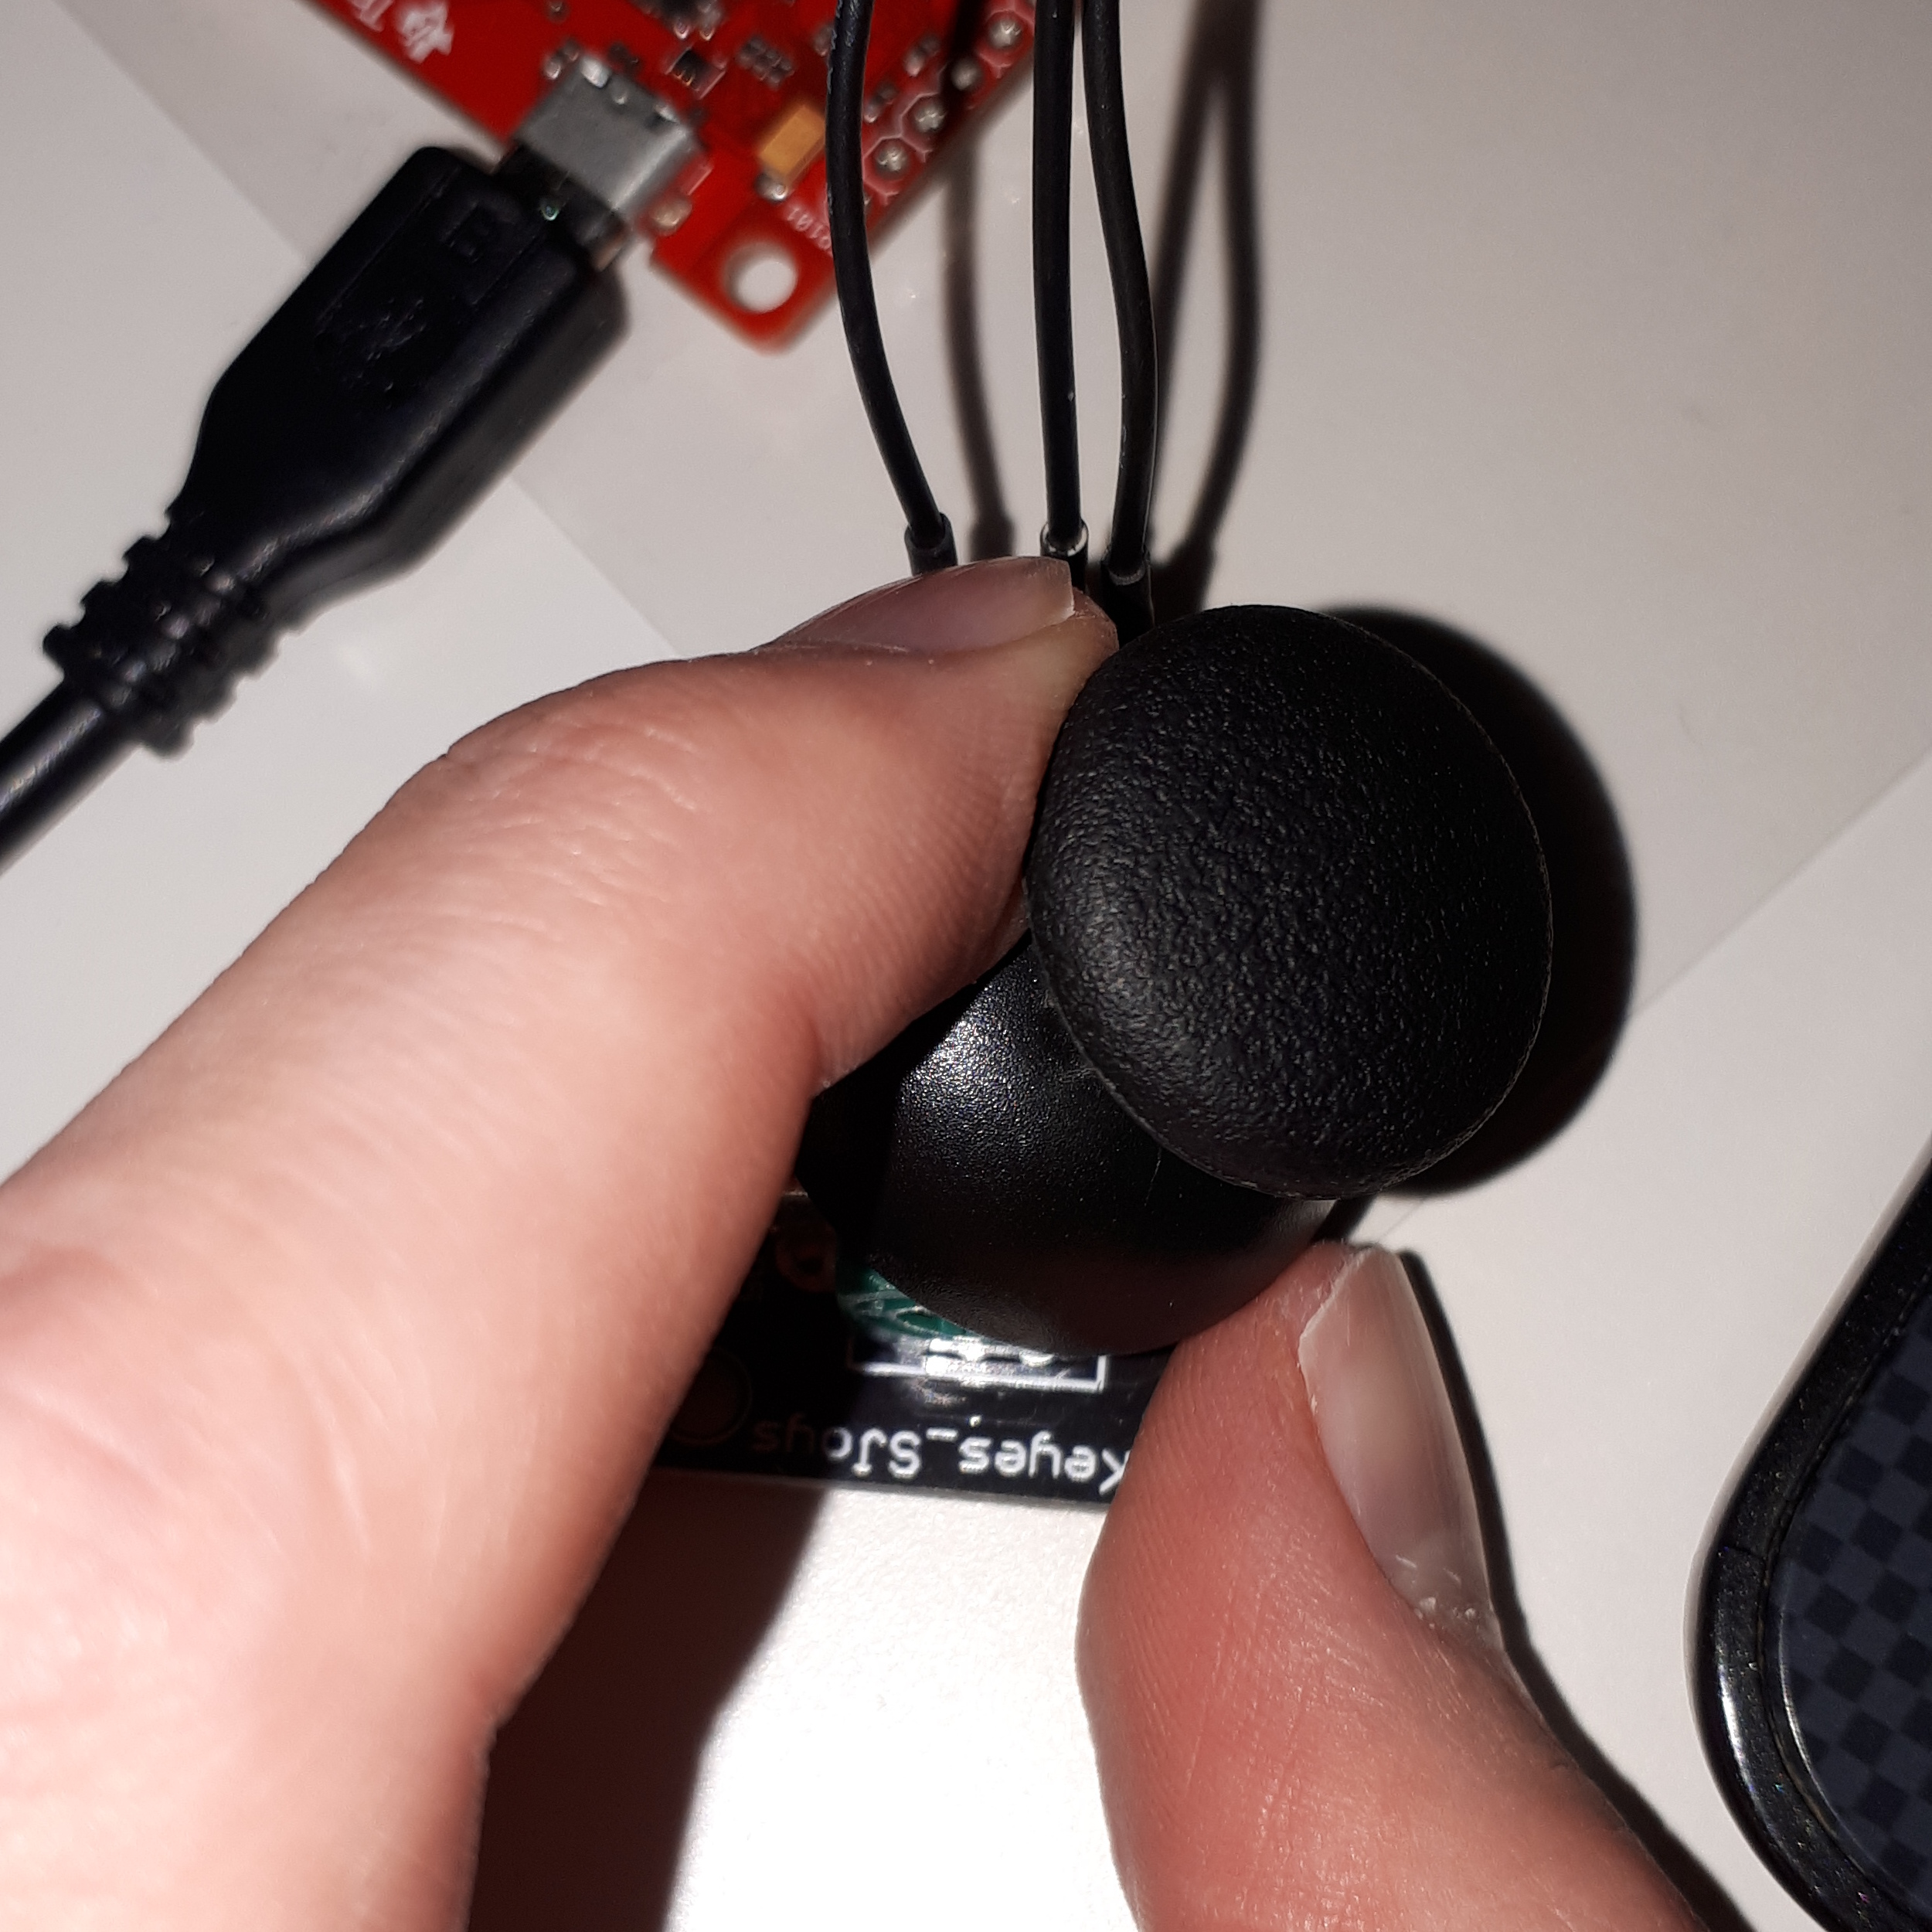
\includegraphics[width=.24\textwidth]{in_lo} & 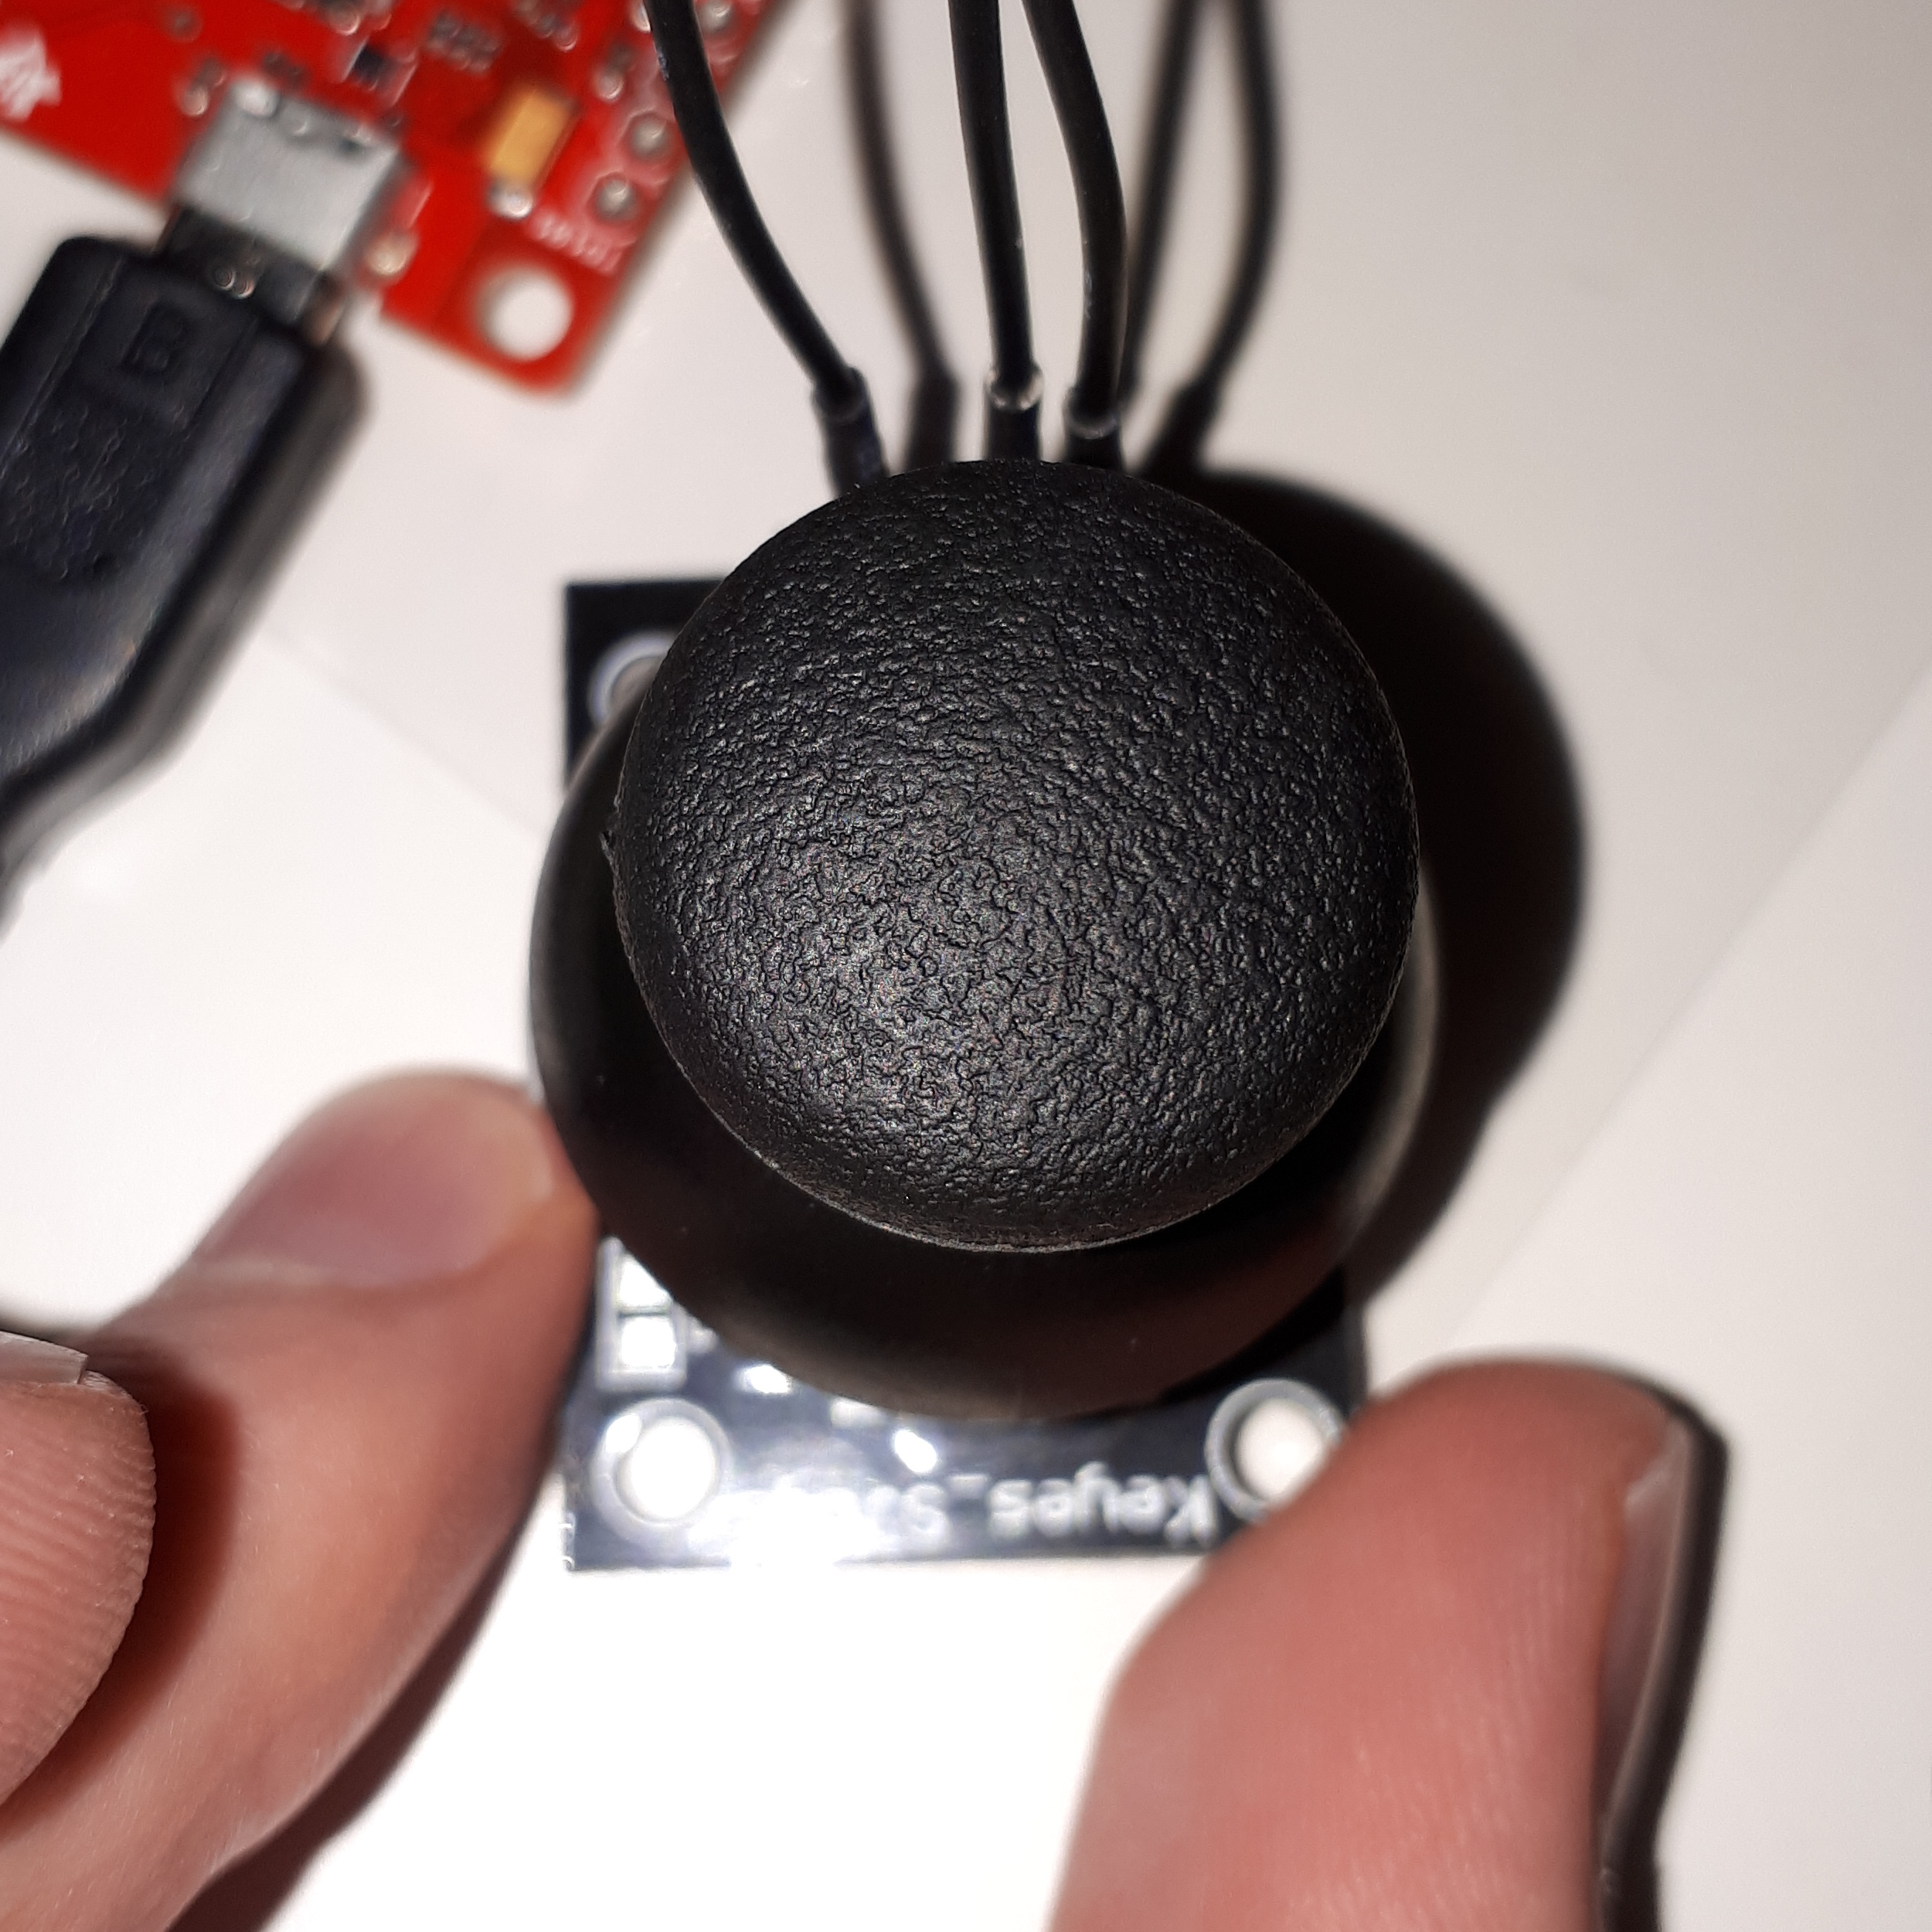
\includegraphics[width=.24\textwidth]{in_n} & 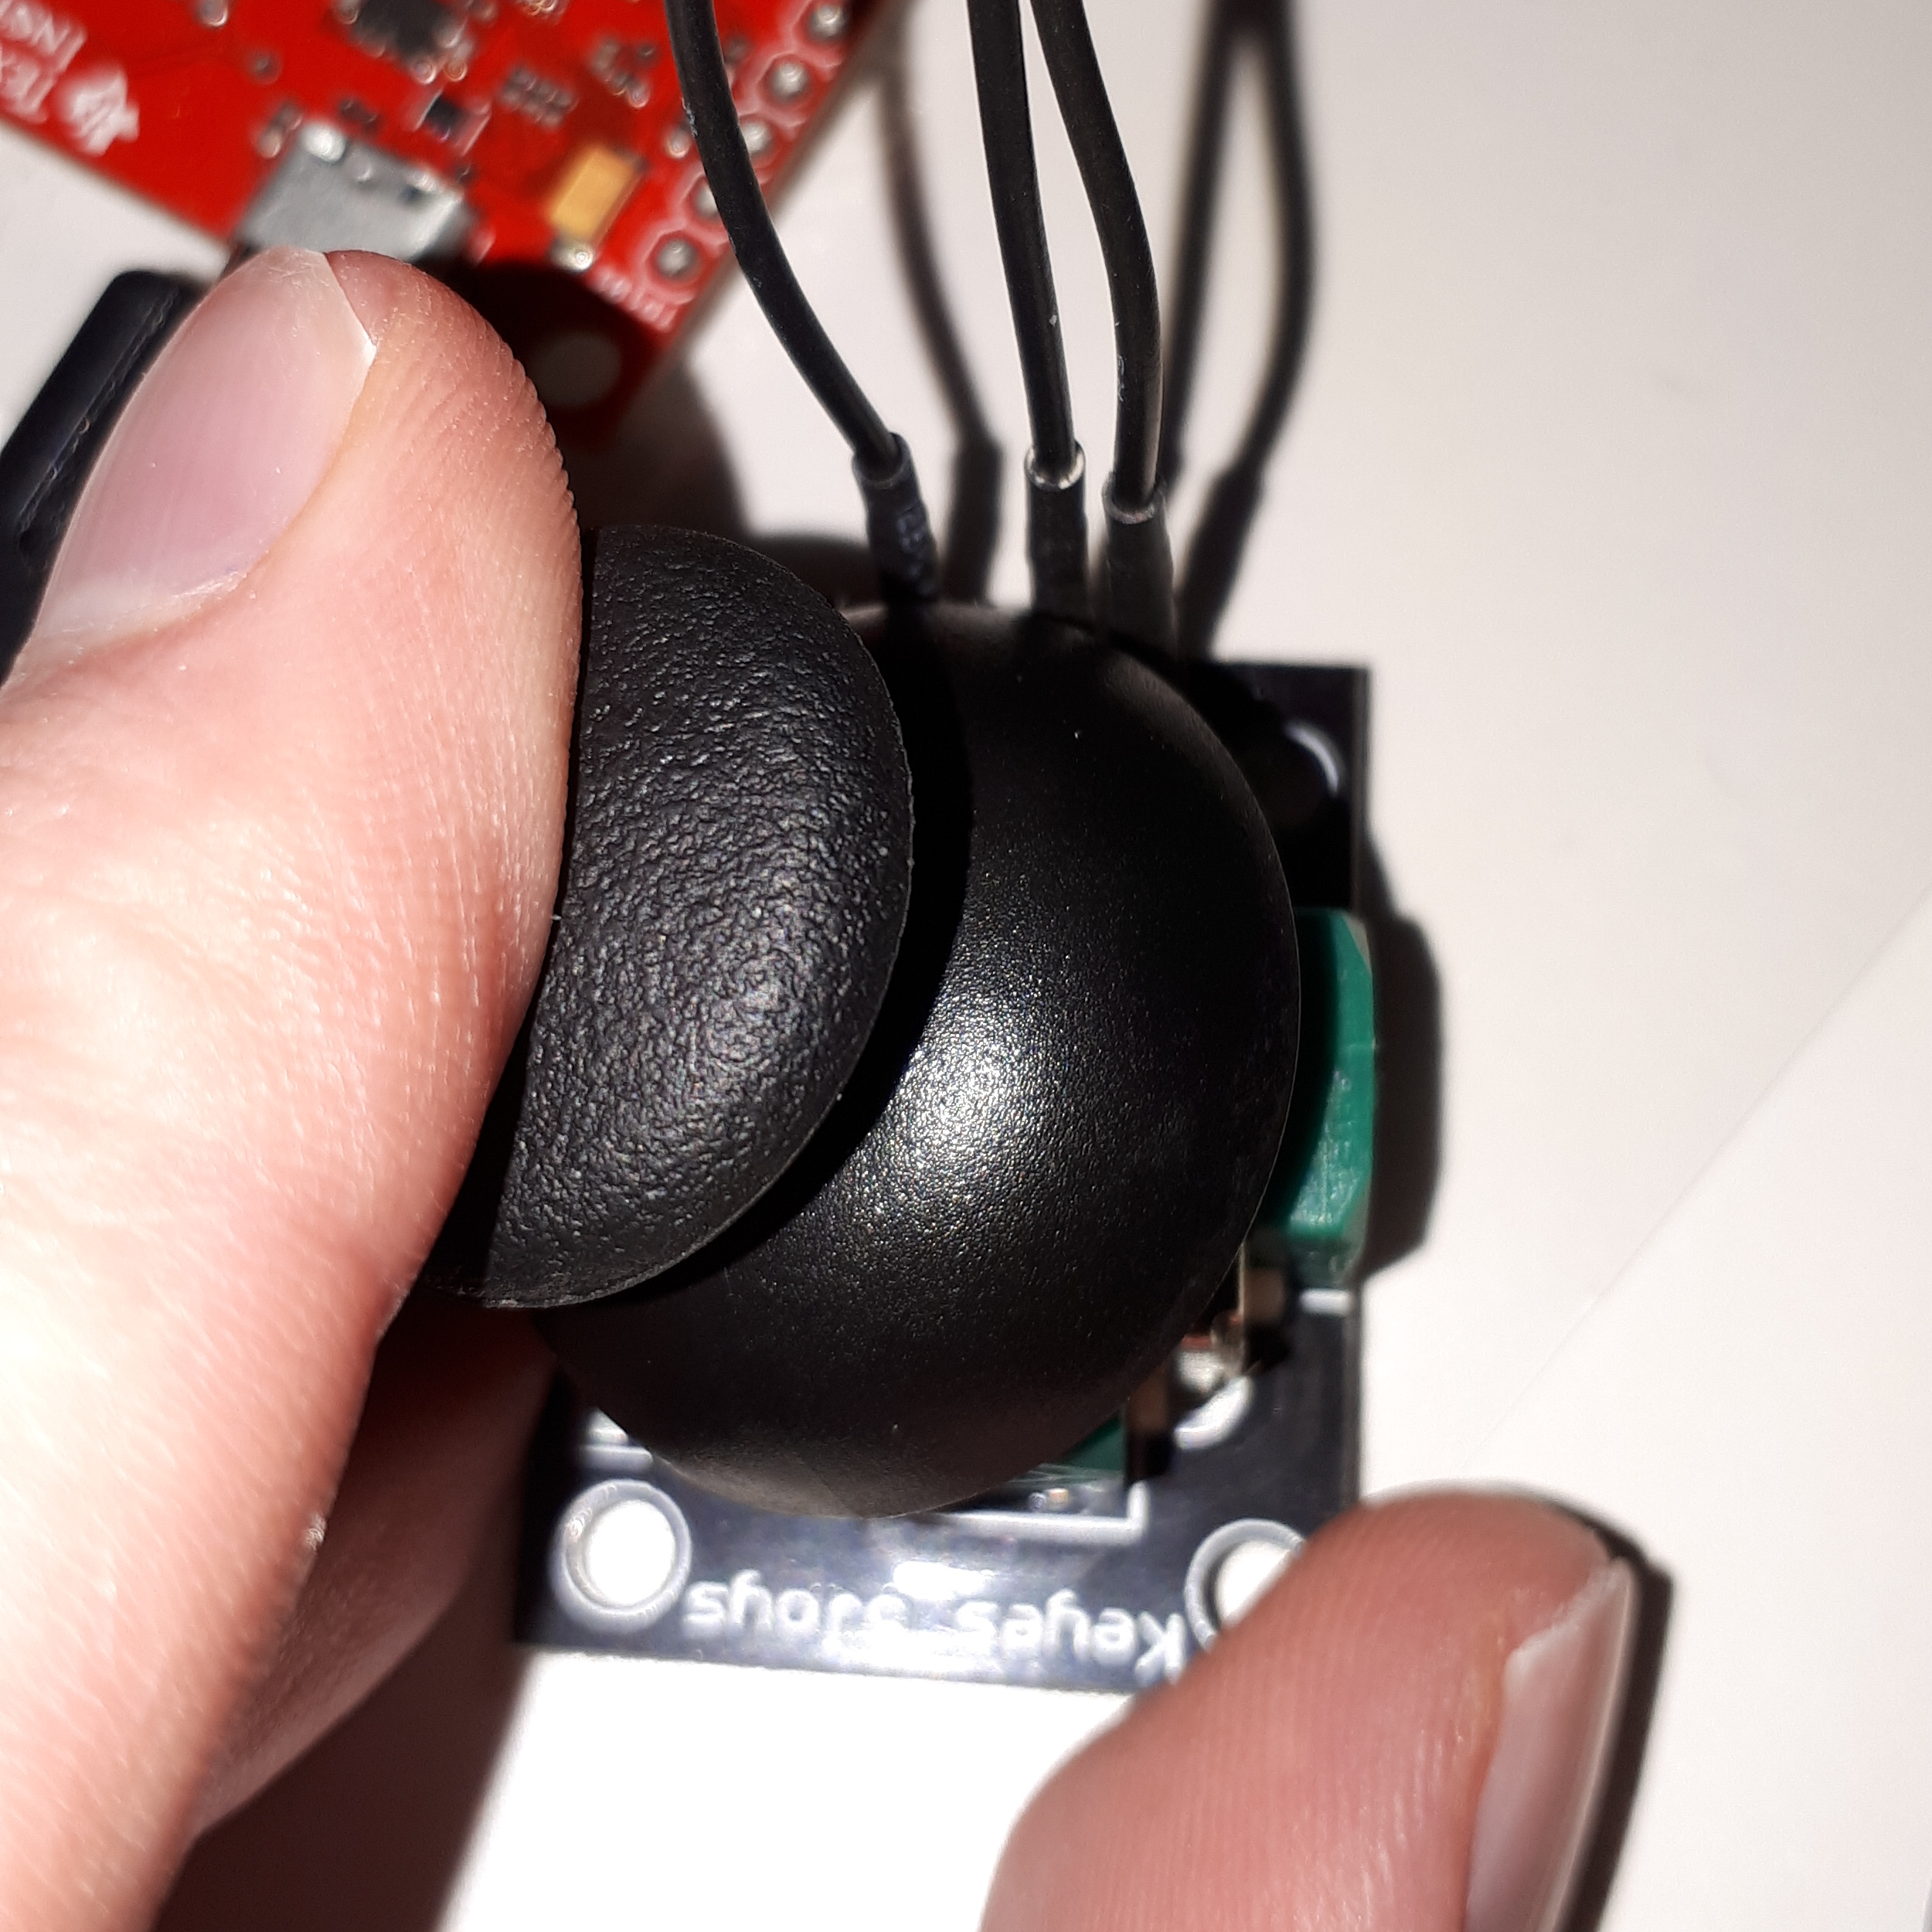
\includegraphics[width=.24\textwidth]{in_hi} \\ 
		\hline 
		Sampled value & 0 -- 9 & 8428 -- 8433 & 16369 -- 16373 \\ 
		\hline 
		PWM & 
			\multilinecell{Width: \SI{0.9955}{\milli\s}\\Period: \SI{19.91}{\milli\s}
				\\Duty cycle: 5.000\%
				\\(Figure \ref{fig:pwmlow})} & 
			\multilinecell{Width: \SI{1.507}{\milli\s}\\Period: \SI{19.91}{\milli\s}
				\\Duty cycle: 7.569\%
				\\(Figure \ref{fig:pwmneutral})} & 
			\multilinecell{Width: \SI{1.990}{\milli\s}\\Period: \SI{19.91}{\milli\s}
				\\Duty cycle: 9.995\%
				\\(Figure \ref{fig:pwmhigh})}  \\ 
		\hline 
		Result & 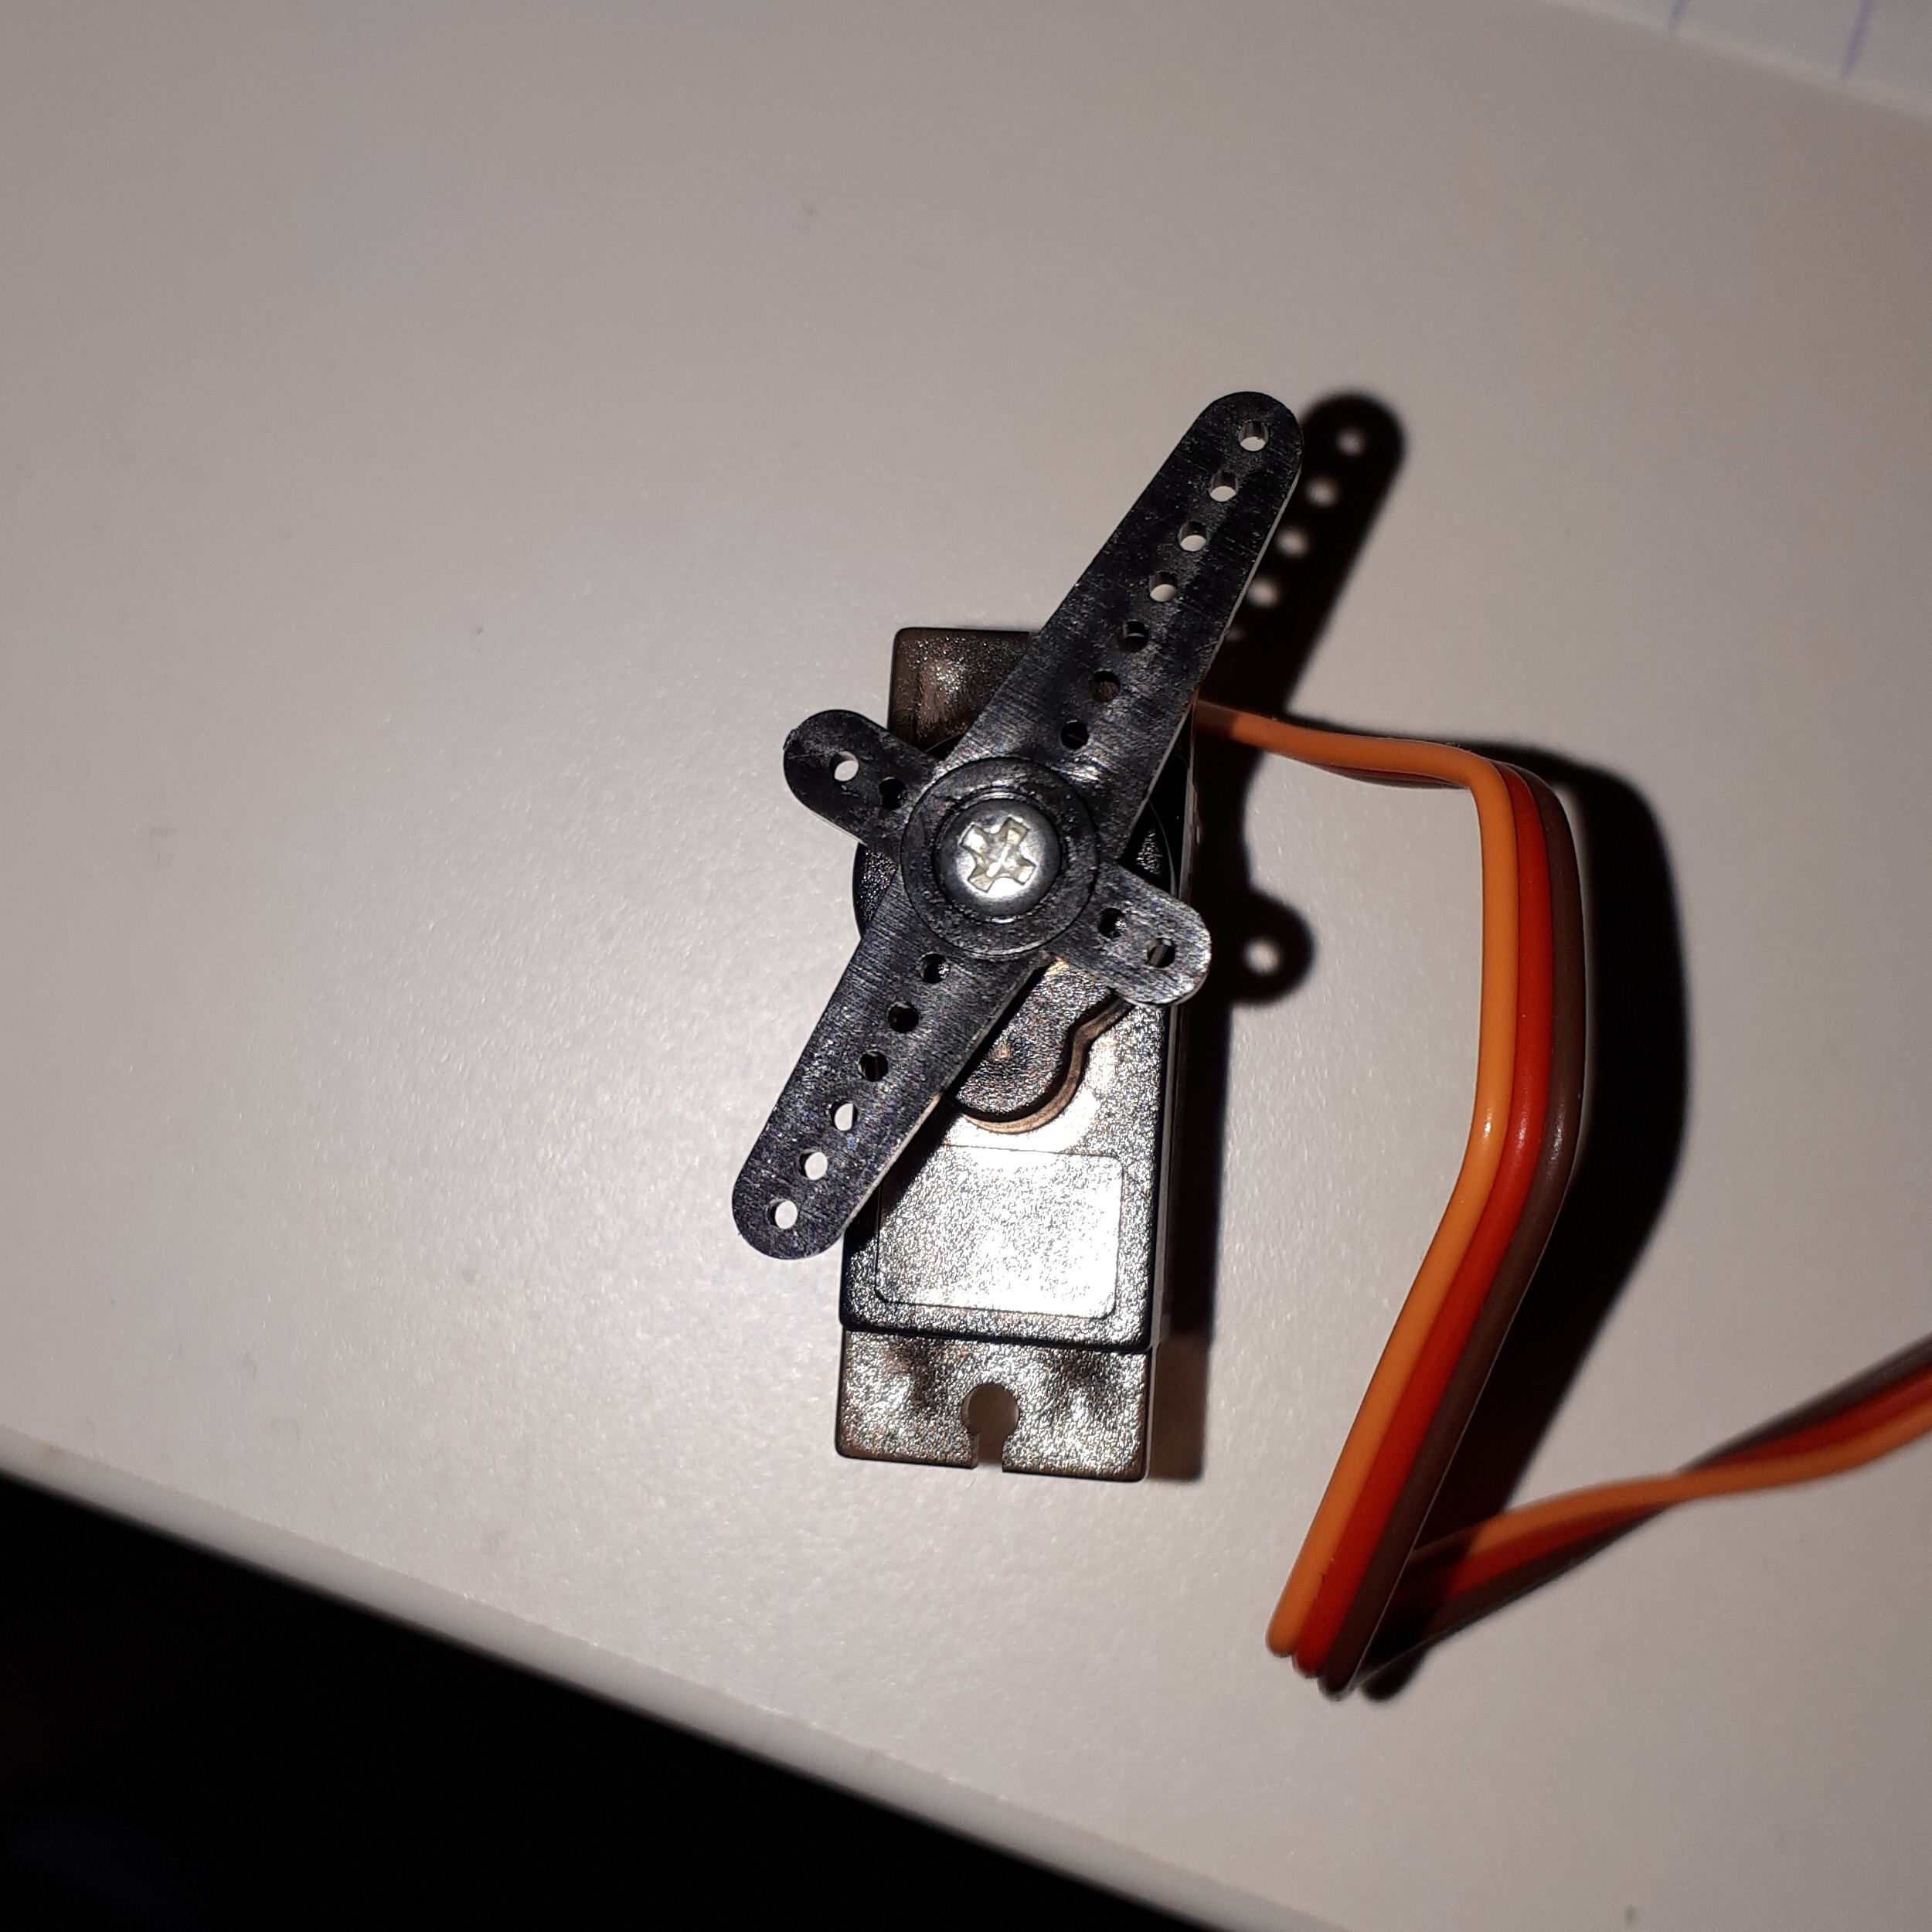
\includegraphics[width=.24\textwidth]{out_lo} & 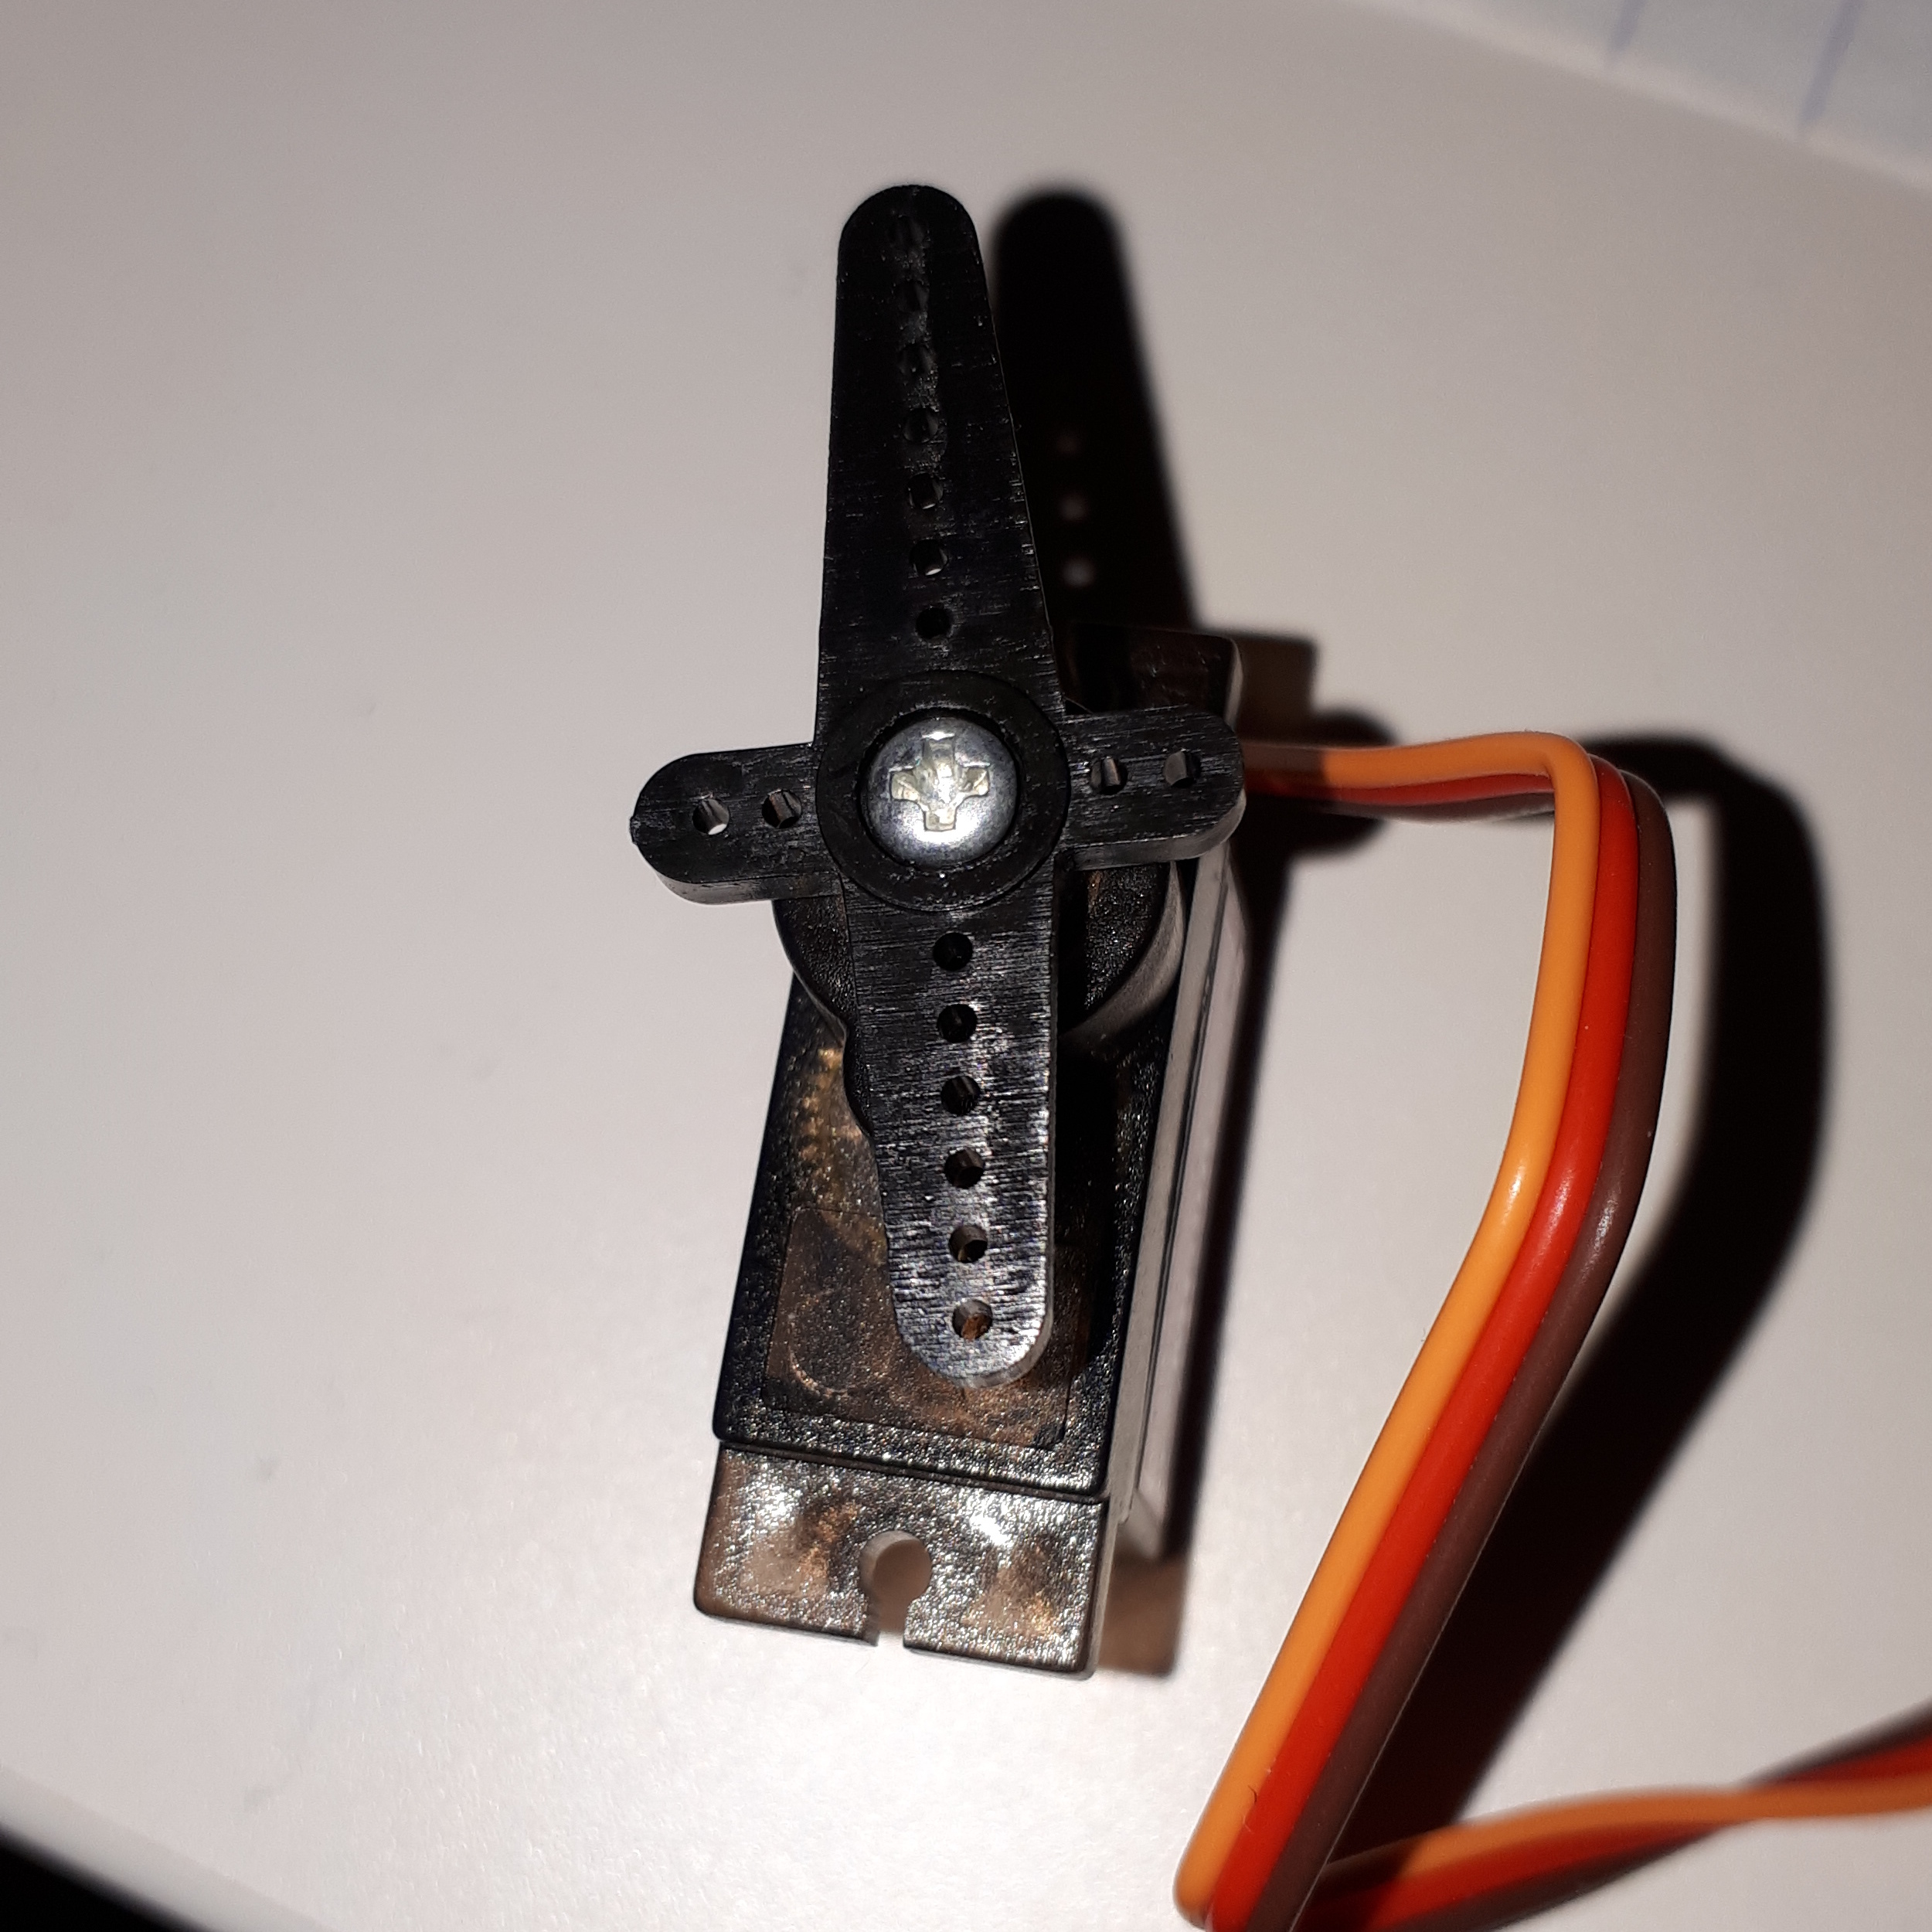
\includegraphics[width=.24\textwidth]{out_n} & 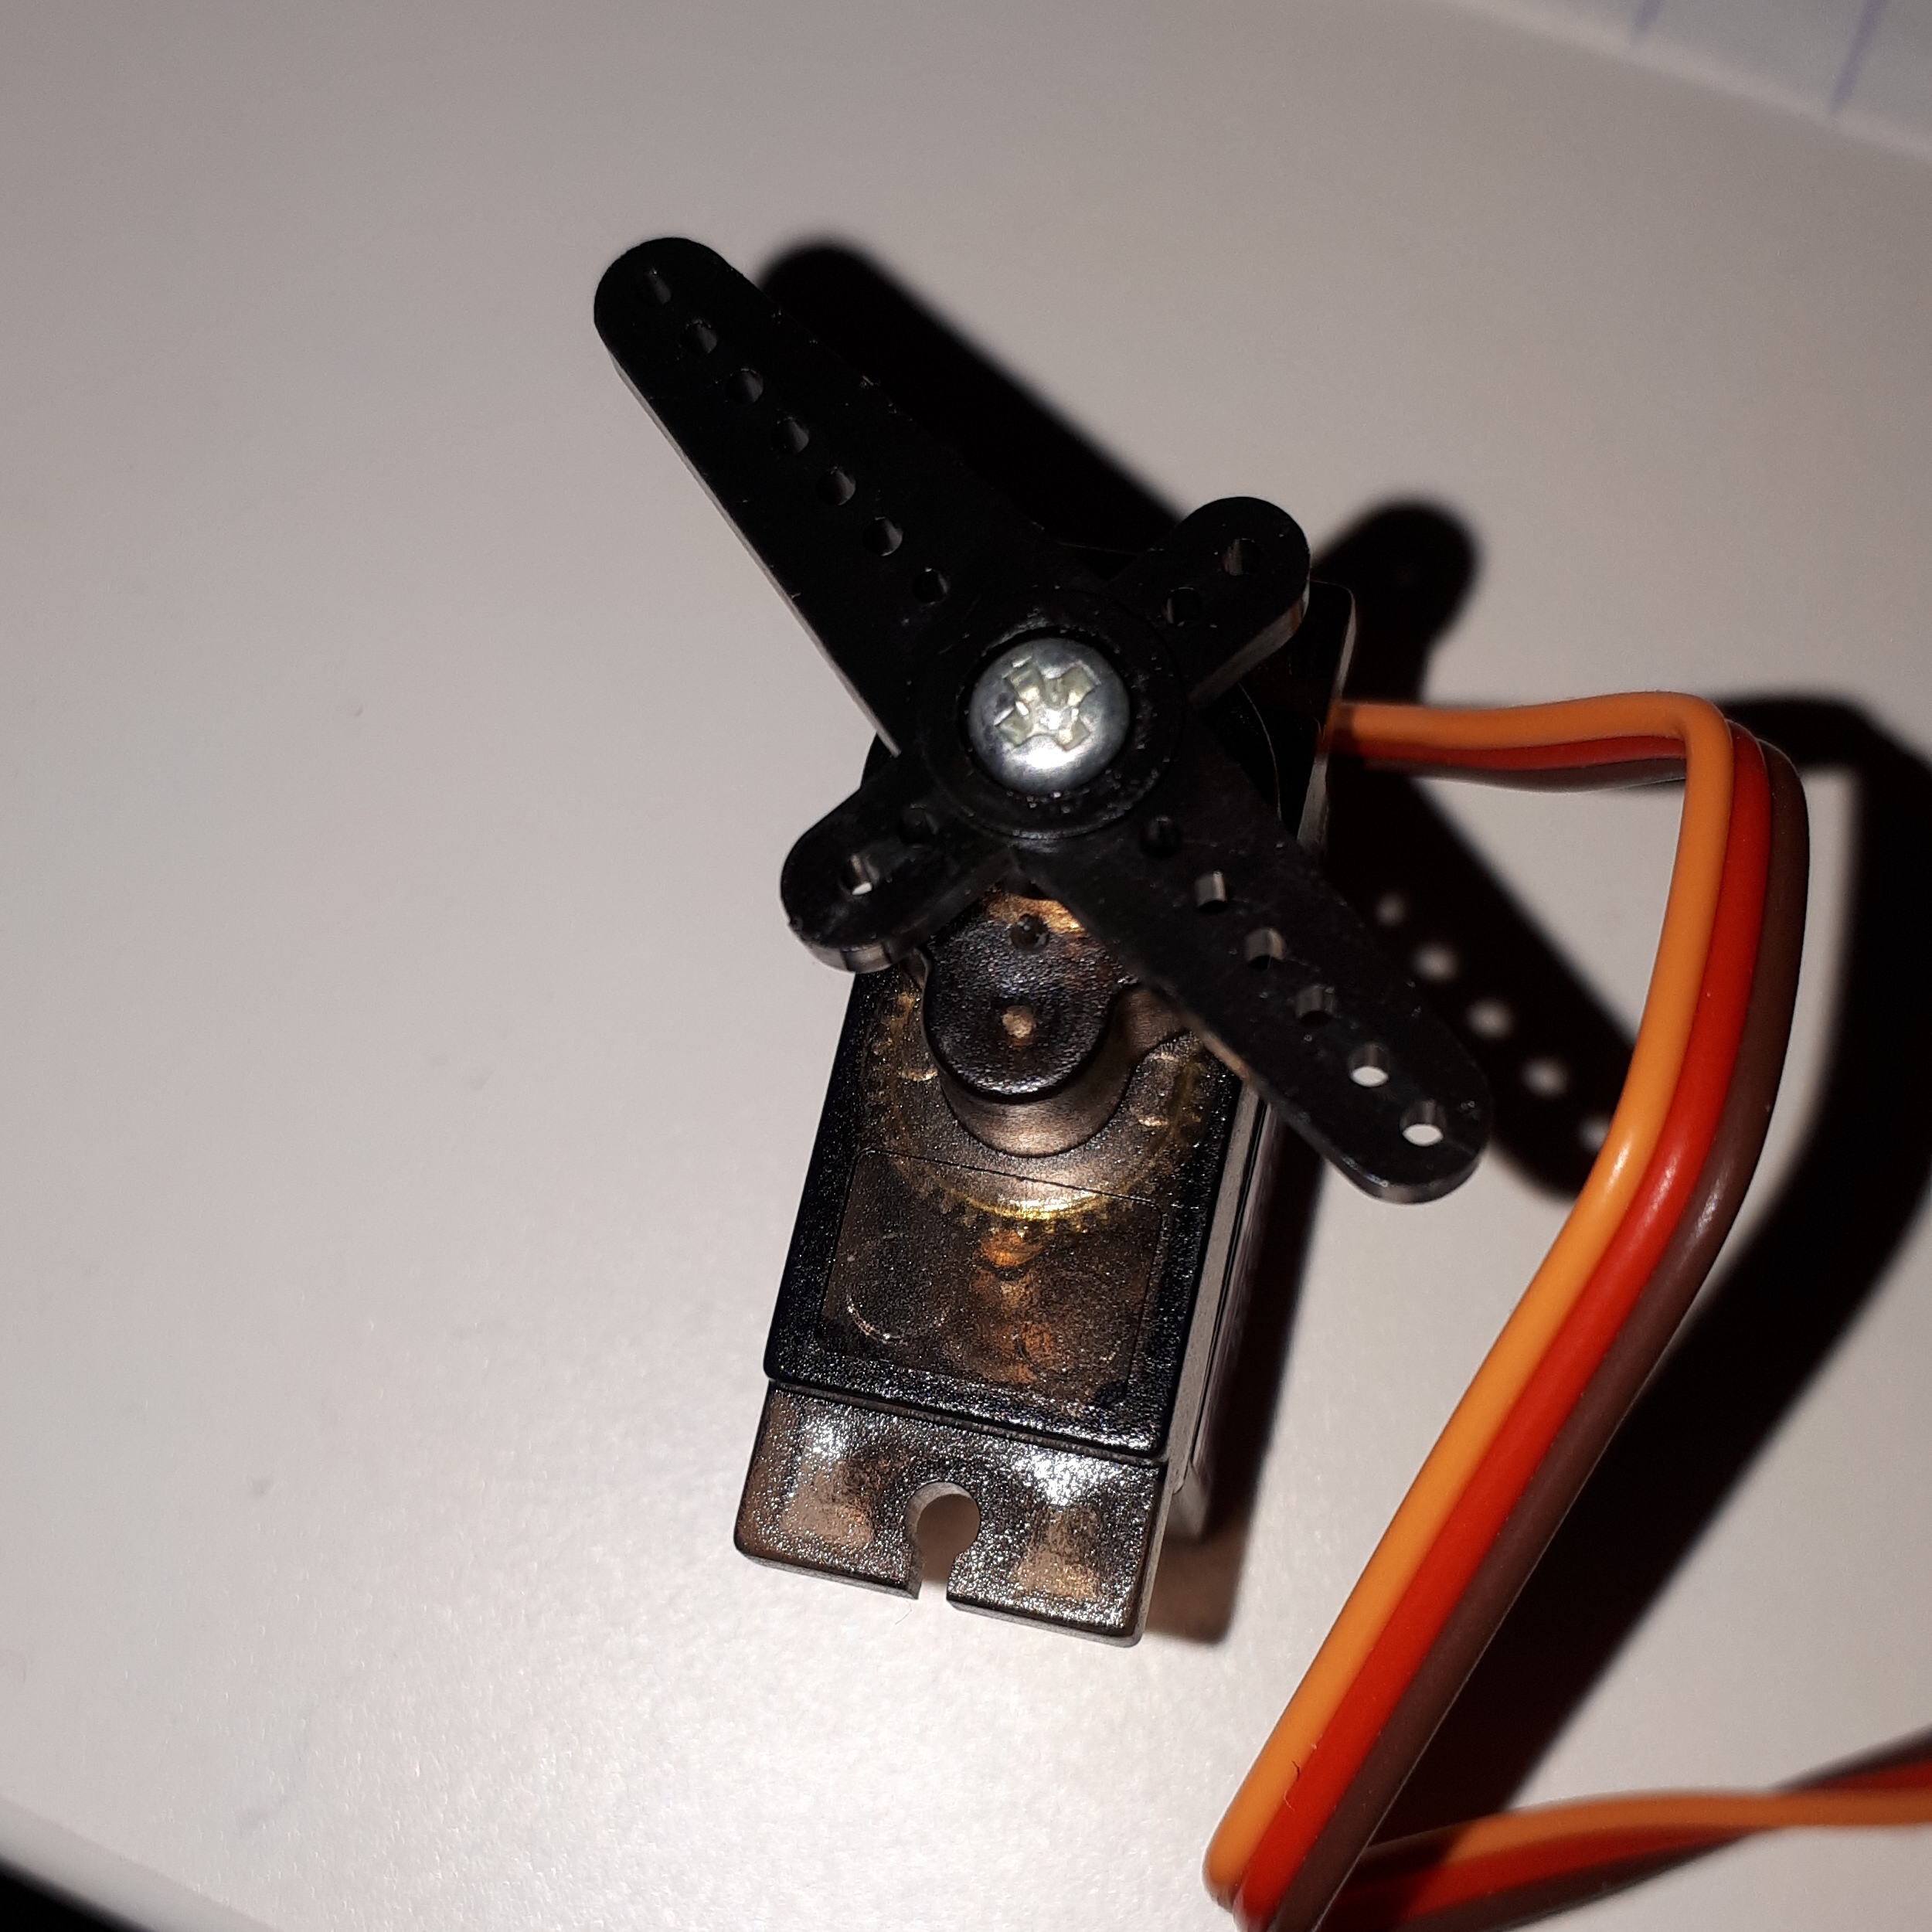
\includegraphics[width=.24\textwidth]{out_hi}\\
		\hline
	\end{tabular} 
	\caption{Inputs \& results in three simple cases}
	\label{tab:results}
\end{table}

\begin{figure}[h]
	\centering
	\begin{subfigure}{\textwidth}
		\centering
		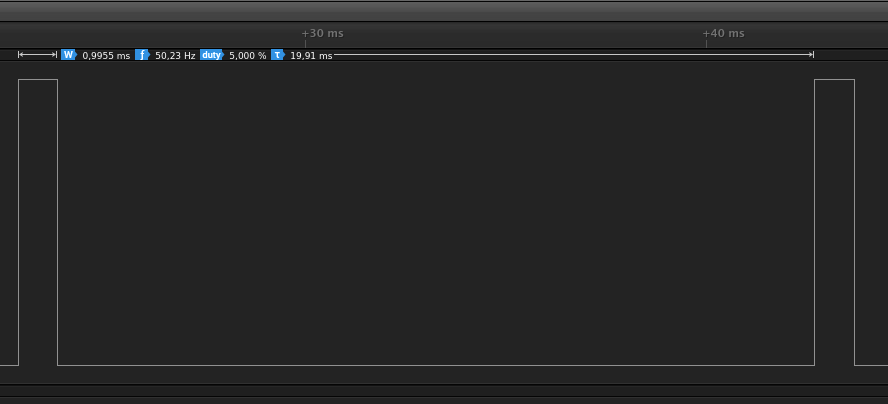
\includegraphics[width=.9\linewidth]{pwm_low}
		\caption{PWM for minimum input}
		\label{fig:pwmlow}
	\end{subfigure}
	\begin{subfigure}{\textwidth}
		\centering
		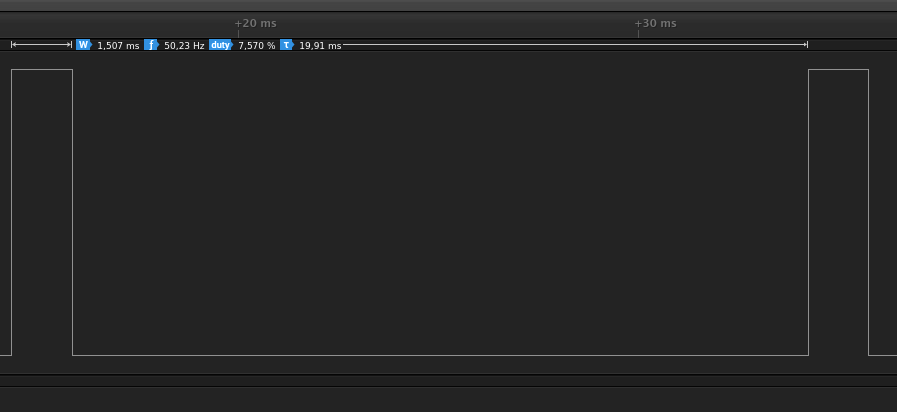
\includegraphics[width=.9\linewidth]{pwm_neutral}
		\caption{PWM for neutral input}
		\label{fig:pwmneutral}
	\end{subfigure}
	\begin{subfigure}{\textwidth}
		\centering
		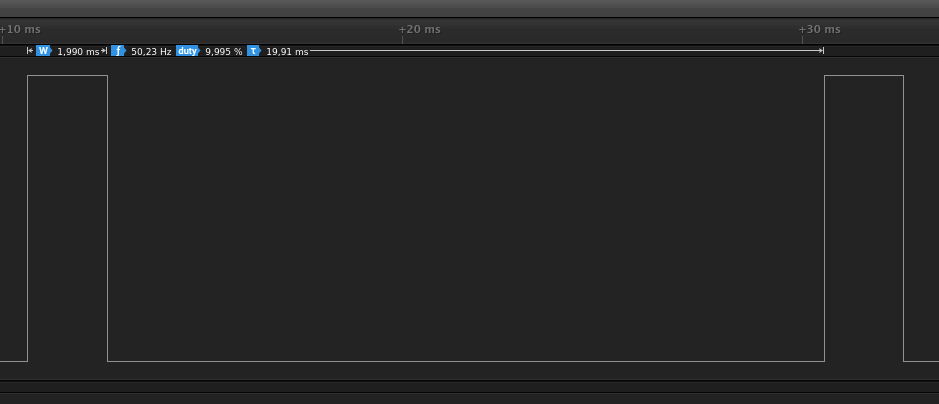
\includegraphics[width=.9\linewidth]{pwm_high}
		\caption{PWM for maximum input}
		\label{fig:pwmhigh}
	\end{subfigure}
	\caption{PWM on pin 2.4 for three different inputs}
	\label{fig:pwm}
\end{figure}

\subsection{Precision considerations}

During this whole lab, I decided to target a precision of 1\%.

We can immediately note that the period of the PWM is \SI{19.91}{\milli\s} for an expected \SI{20}{\milli\s}, meaning an error of 0.5\%. Thus the clock system and timer block respect the targeted precision.

The sampled values cover almost the whole range of the 14-bit ADC; however the maximum value doesn't quite reach $2^{14}-1 = 16383$. I believe this is simply due to the potentiometer's range, but I haven't been able to verify its output voltage. Also, the neutral position doesn't seem to correspond exactly to $V_{cc}/2$, and this is reflected on the PWM width.

The PWM width ranges from \SIrange{0.9955}{1.990}{\milli\s}, which corresponds to the expected \SIrange{1}{2}{\milli\s} range with a precision of 0.5\%.

\section{Conclusion}

The analog voltage of the joystick is sampled every \SI{50}{\milli\s} by the 14-bit ADC and is used to determine the width of the output PWM. This PWM respects the constraints (period of \SI{20}{\milli\s} with a width of \SIrange[range-phrase=--,range-units=single]{1}{2}{\milli\s}) with a precision better than 1\%.

The servomotor is correctly controlled by the joystick. It reacts quickly to changes in joystick position, and the resolution of its angle also seems satisfactory. You can see the system working in the demo video.

\end{document}